\chapter{Implementarea aplicației}

\section{Tehnologii folosite pentru aplicația client}

\subsection{JavaScript}

JavaScript este un limbaj de programare ce permite realizarea de funcționalități complexe pentru paginile web. A fost lansat în 1995 sub numele de LiveScript \cite{brandan_eich_js} și și-a făcut un renume, fiind, în 2021, cel mai popular limbaj de programare, conform unui chestionar realizat de către Stack Overflow \cite{js_stackoverflow}. Reușita JavaScript-ului vine atât din eficiența prin care reușește să dinamizeze paginile web, dar și prin ecosistemul de librării create în jurul său. Librăriile bazate pe JavaScript sunt în continuă dezvoltare și creștere, astăzi existând mai mult de un milion de librării listate oficial \cite{number_of_js_libraries}.

\subsection{React}

Așa și cum apare pe pagina oficială, React nu este nimic mai mult decât o librărie pentru realizarea interfețelor \cite{react_webpage}. A fost creat de către Jordan Walke, un inginer al companiei Facebook, în 2011 și implementat în newsfeed-ul platformei în același an, urmând ca, mai târziu, când Facebook a achiziționat Instagram, să fie implementat și acolo. Cu timpul, React s-a dezvoltat, iar, în 2013, a devenit open source, fapt ce a dus la o dezvoltare exponențială în materie de capabilități și funcționalități pe care le poate realiza. Astăzi, React este cea mai populară soluție pentru interfața unei aplicații web \cite{popularity_of_react}.

\newpage

\begin{figure}[!ht]
    \centering
    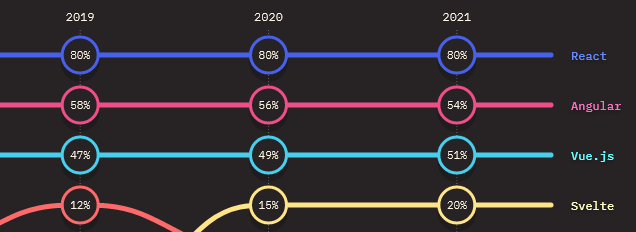
\includegraphics[width=135mm]{images/react_popularity.png}
    \caption{Clasament \enquote{State of JavaScript} pentru librăriile de frontend, după utilizare}
\end{figure}


Eficiența librăriei este realizată de un cumul de factori precum:

\begin{itemize}
    \item Componente reutilizabile. Aceste componente reprezintă unul din cele mai importante concepte în React, permițând reutilizarea acestora oriunde în aplicație. Ele pot fi customizate ușor, dat fiind că acceptă parametrii când vine vorba de procesat starea internă și de afișat informații.
    
    \item DOM Virtual. Pentru a eficientiza schimbările rapide pe care le realizează librăria, React are implementat un DOM virtual, adică o copie mai \enquote{lightweight} a DOM-ului real. Operațiile de schimbare ale DOM-ului real sunt lente, astfel, React poate updata numai componentele care sunt alternate, neavând nevoia de a redesena tot DOM-ul.
    
    \item Curs de date unidirecțional. React urmează un curs de date unidirecțional, astfel, când este dezvoltată o aplicație React, deseori componentele sunt așezate într-un mod \enquote{parent-child}, astfel informația trecând de la componenta părinte la componenta copil într-un mod direct.
    
    \item Tool-uri dedicate pentru debugging. Facebook a lansat o extensie open source pentru browser ce are ca scop principal inspectarea componentelor React și a ierarhiei acestora direct din browser.
    
\end{itemize}

Astfel, am folosit toți acești factori în realizarea aplicației Voting App, începând de la cele mai mari componente (componenta \enquote{Route}) până la cele mai mici (butoane, texte, inputuri, etc.).

\subsection{NPM}

Node Packet Manager (NPM) reprezintă, în același timp, 2 concepte diferite. În primul rând este cel mai mare registru online pentru publicarea pachetelor open source realizate în Node.js și, în al doilea rând, este un modul ce suplimentează linia de comandă cu mai multe instrucțiuni, astfel încât să fie posibilă interacțiunea cu registrul online pentru ajutarea, atât în instalarea pachetelor necesare unui proiect, cât și pentru gestionarea versiunii și dependențelor pachetelor \cite{what_is_npm}.

Pentru a folosi React, este necesară o multitudine de pachete ce trebuie instalate cu ajutorul NPM. Aceste pachete sunt salvate în directorul \enquote{node\_modules}, iar versiunea lor în fișierul \enquote{package{.}json} sub tag-ul \enquote{dependencies}. Instalarea pachetelor s-a efectuat utilizând comanda \enquote{npm install nume\_pachet}.

\subsection{Axios}

Axios este o simplă librărie de JavaScript ce ajută la realizarea request-urilor HTTP de pe client \cite{axios_docs}. Librăria este bazată pe conceptul de \enquote{Promisiune}. O promisiune reprezintă o eventuală completare sau un eventual eșec al unei operații asincrone și a valorii returnate de către aceasta \cite{what_is_promise}.

În Voting App am folosit o instanță definită pentru client, astfel încât adresa IP la care sunt făcute request-urile către aplicația backend să fie modificată ușor.

\begin{code}
\begin{minted}[bgcolor=bg,frame=lines,framesep=2mm,fontsize=\footnotesize,baselinestretch=1]{js}
export default axios.create({
    baseURL: 'http://127.0.0.1:8000',
    headers: {
        "Content-type": "application/json"
    }
});
\end{minted}
\captionof{figure}{Clientul Axios pentru Voting App}
\label{code:axios-code}
\end{code}
\hfill

De asemenea, pentru a putea oferi aplicației de backend o modalitate de a identifica persoana de unde a fost făcut un request, se va trimite, pe lângă datele request-ului, și un token. Acest token este trimis în header-ul request-ului și este primit de către utilizator atunci când este făcută autentificarea. În funcție de acest token, serverul poate identifica dacă un utilizator are rol de admin sau nu și poate bloca un request făcut pe o cale protejată dacă utilizatorul nu îndeplinește acest criteriu.

Pentru a putea realiza diferența dintre tipurile de răspunsuri primite atunci când este făcut un request, aplicația de backend va trimite și un cod HTTP. Aceste coduri se împart în următoarele categorii \cite{http_codes}:

\begin{itemize}
    \item Răspunsuri informative (100–199)
    \item Răspunsuri de succes (200–299)
    \item Mesaje de redirecționare (300–399)
    \item Erori de client (400–499)
    \item Erori de server (500–599)
\end{itemize}

În funcție de codul primit, aplicația de frontend observă dacă request-ul făcut a avut succes sau nu și va reacționa ca atare.

\subsection{Redux}

Redux este o librărie de JavaScript menită să gestioneze state-ul în aplicație. A fost creat în 2015 de către Dan Abramov și Andrew Clark și este cea mai des folosită librărie pentru acest lucru. Modul în care funcționează Redux este unul relativ simplu. Este creat un \enquote{store} central în care este ținut intregul state al aplicației. Fiecare componentă poate accesa acest \enquote{store} fără a avea nevoie de informații suplimentare, funcționând asemănător unor variabile globale \cite{redux_docs}. Există trei componente principale ce formează Redux, și anume:

\begin{itemize}
    \item Actions, reprezintă event-uri ce pot modifica state-ul. Ele sunt singura modalitate prin care se pot trimite date către \enquote{store} în cadrul unei metode \enquote{dispatch}. Există mai multe tipuri de acțiuni și, de aceea, ele sunt nevoite să conțină o proprietate \enquote{type}.
    \item Reducers, funcții ce iau state-ul curent al aplicației, aplică o acțiune și întorc tot un state. Ele sunt folosite pentru gestionarea continua a variabilelor ce se pot modifica pe parcursul utilizării aplicației.
    \item Store, fiind obiectul central în care sunt salvate datele. Pentru ca o componentă să aibă acces la acestea, aplicația a fost pusă într-un provider în care au fost definite stările inițiale.

\end{itemize}

În cadrul Voting App am folosit Redux pentru a gestiona două state-uri diferite. Primul state conține date despre autentificare - dacă există un utilizator autentificat pe platformă și token-ul pe care acesta l-a primit din aplicația de backend atunci când a fost făcută autentificarea. Al doilea state pe care Redux l-a gestionat în Voting App este cel al utilizatorului autentificat, în care sunt salvate date precum: identificatorul utilizatorului, numele și prenumele acestuia, adresa de email, grupul din care face parte și nu numai. De asemenea, în cadrul aplicației au fost definite acțiuni care vizează login-ul și logout-ul de pe platformă și schimbarea datelor personale.

\subsection{Chakra UI}

O aplicație modernă are nevoie și de o stilizare ca atare și consistentă. Pentru a îmbunătății acest proces și pentru a oferi utilizatorului o experiență cât mai intuitivă pe platformă a fost folosită librăria Chakra UI. Această librărie permite dezvoltatorilor utilizarea unor componente deja stilizate și posibilitatea de a stiliza propriile componente într-un mod foarte rapid și eficient din punct de vedere al timpului necesar. Unul dintre principalele avantaje ale Chakra UI față de alte librării de stilizare este modul în care elementele reacționează la diferite rezoluții și ecrane (de la mobil și tabletă până la desktop), fiind o librărie \enquote{responsive}. A fost realizată de către Segun Adebayo și are peste 26 de mii de star-uri pe GitHub \cite{chakra_github}. Un alt avantaj al acestei librării este dat de ușurința cu care poate fi realizată o temă proprie - este suficientă doar descrierea unui obiect în care sunt puse culorile și măsurătorile dorite, librăria dispunând și de o implementare ușoară a unui \enquote{dark theme}.

Pentru a accesa componentele dispuse de către Chakra UI, este necesară punerea aplicației într-un provider numit \enquote{ChakraProvider}, asemenea provider-ului librăriei Redux. În Voting App, toate componentele sunt stilizate utilizând proprietăți ale librăriei, ca de exemplu: \enquote{mr} pentru a seta marginea la dreapta a unei componente sau \enquote{borderRadius} pentru a curba marginea unui element.

De asemenea, au fost folosite componente prestabilite, în special pentru input-urile din formulare, deoarece librăria dispune de un ecosistem bine definit pentru ceea ce înseamna \enquote{user feedback} atunci când vine vorba de validare.

Meniul principal al Voting App este realizat utilizând un Flexbox \cite{flexbox}, iar cartonașele ce reprezintă buletinele de vot conțin Box-uri stilizate pentru a oferi un efect de umbră. În același sens, la baza fiecărei pagini se află un layout de standard. Acest layout este alcătuit din:

\begin{itemize}
    \item Navbar. Reprezintă partea de sus a layout-ului și conține, pentru desktop, doar un buton cu numele utilizatorului astfel ca, atunci când este apăsat, să deschidă un meniu cu două opțiuni: pagina de setări și deconectare. Pentru mobil, această componentă afișează un al doilea buton, de tip \enquote{burger}, care deschide utilizatorului Sidebar-ul (acesta fiind ascuns din start pe mobil).
    \item Sidebar. Conține toate rutele de bază pe care utilizatorul le poate accesa pentru a vizualiza și a prelucra date în cadrul aplicației (pagina principală, pagina cu toate voturile disponibile, pagina cu toate grupurile active și dashboard-ul pentru administrator, în cazul în care utilizatorul are acest rol). Pentru mobil, acesta este ascuns și trebuie deschis prin apăsarea butonului din Navbar. De asemenea, atunci când utilizatorul se află pe mobil, Sidebar-ul dispune de un buton suplimentar pentru închiderea sa.
    \item Titlebar. Este alcătuit din două elemente - numele paginii curente și un buton care redirecționează utilizatorul cu un pas înapoi pe aplicație.
    \item Footer. Conține două link-uri care duc la pagina principală a site-ului facultății și la pagina oficială de contact al secretariatului facultății.
\end{itemize}

\hfill

\begin{figure}[!h]
    \centering
    
\includegraphics[width=135mm]{images/navbar_desktop.png}
    \caption{Navbar pe desktop. În stânga, fiind începutul Sidebar-ului}
\end{figure}

\begin{figure}[!h]
    \centering
    
\includegraphics[width=115mm]{images/navbar_mobil.png}
    \caption{Navbar pe mobil, cu butonul \enquote{burger}}
\end{figure}


\section{Tehnologii folosite pentru aplicația server}

\subsection{Python}

Python este un limbaj de programare interpretat, orientat pe obiecte, ce excelează prin lizibilitatea codului și versatilitate. A fost creat de către Guido Van Rossum, iar prima versiune oficială a fost lansată în anul 1994. Încă de atunci a fost supus unor schimbări și îmbunătățiri constante, dat fiind că în anul 2000 a fost lansată versiunea 2.0 a limbajului, iar, mai recent, în 2008, versiunea 3.0. Conform unei statistici independente \cite{popularity_of_python}, Python ocupa, în sfertul al patrulea al anului 2021, poziția întâi în numărul de apariții în repository-urile de pe GitHub, acest fapt dovedind popularitatea limbajului.

\begin{figure}[!h]
    \centering
    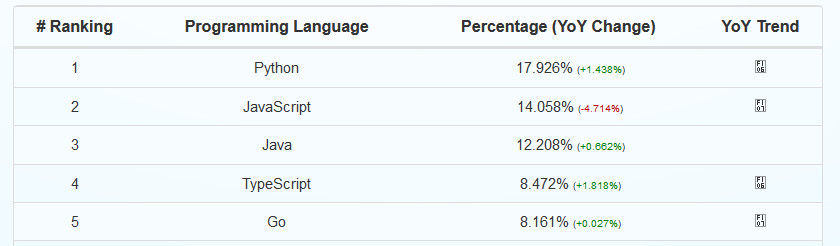
\includegraphics[width=140mm]{images/python_popularity.png}
    \caption{Popularitatea limbajelor de programare pe GitHub}
\end{figure}

Față de alte limbaje de programare precum C și C++, unde este necesară compilarea codului pentru a putea fi executat, adică traducerea codului scris în limbaj mașină ce poate fi executat direct pe CPU, Python funcționează împreună cu un interpretor. Acest interpretor preia codul scris și îl transformă în bytecode, astfel încât să poată fi rulat de către acesta. Această abordare vine cu un set de avantaje, printre care se numără:

\begin{itemize}
    \item Portabilitate. Atunci când un program este scris într-un limbaj ce necesită compilare, acest proces devine specific pentru device-ul pe care este executat compilatorul. În schimb, interpretorul funcționează în același mod pe toate sistemele de operare, astfel, nu există diferențe între un cod scris în Windows, față de un cod scris în Linux.
    \item Scriere dinamică. Implementarea \enquote{dynamic typing-ului} într-un limbaj compilat este foarte grea și poate duce la generarea multor erori. Totuși, pentru un limbaj interpretat, \enquote{dynamic typing-ul} este implementat de la sine, astfel dezvoltatorii putând să evite declararea tipului unei variabile (int, string, etc.).
    \item Debugging mai rapid. Interpretorul rulează programul linie cu linie și, atunci când întâmpină o eroare, dezvoltatorul știe concret cauza și linia la care a apărut.
\end{itemize}

Pentru Voting App a fost folosită versiunea de Python 3.10.1.

\subsection{Django}

Django este un framework open source pentru backend realizat în Python ce permite dezvoltarea de aplicații web rapid și scalabil. Framework-ul a fost conceput începând cu anul 2003, iar, în 2005 a devenit open source. Încă de atunci, a avut parte de o continuă dezvoltare, atingând, în 2008 versiunea 1.0, iar, în 2022, versiunea 4.0. Unul dintre avantajele Django este simplitatea dezvoltării aplicațiilor, urmând o structură MVC (\enquote{Model, View, Controller}) \cite{MVC_what_is}.

\begin{figure}[!h]
    \centering
    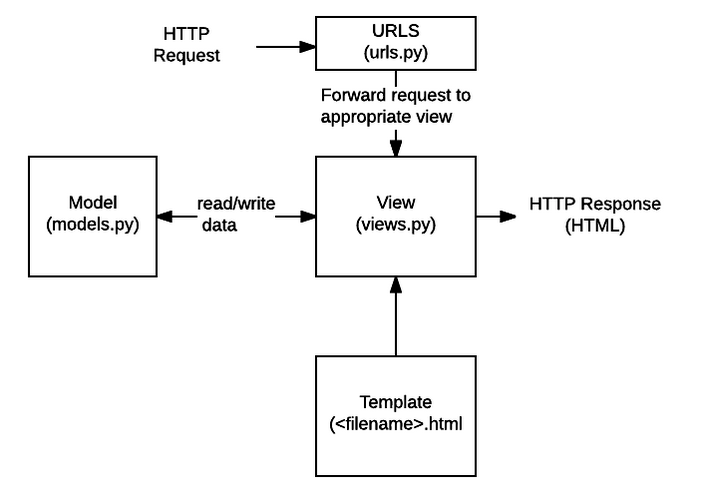
\includegraphics[width=130mm]{images/django.png}
    \caption{Arhitectura framework-ului Django}
\end{figure}

Scopul utilizării Django în Voting App a fost folosirea librăriei Django REST Framework, ce permite utilizarea lui drept un serviciu de API. API (\enquote{Application Programming Interface}) este un mecanism ce permite comunicarea între două componente software utilizând un set de reguli, definiții și protocoale. Arhitectura acestui mecanism este împărțită în client și server - clientul trimite request-uri către server, așteptând un răspuns. Există mai multe tipuri de API, iar cel folosit de Voting App este REST API.

REST (\enquote{Representational State Transfer}) definește un set de operații precum GET, PUT, DELETE, POST, etc. pe care un client le poate accesa pentru a comunica date printr-un protocol HTTP. Cea mai importantă caracteristică a REST este lipsa unei \enquote{stări}, adică serverul nu salvează datele transmise între request-uri. \cite{what_is_rest}. Datele transmise de un REST API sunt de tip text, lipsite de orice elemente grafice sau audio.

\begin{figure}[!h]
    \centering
    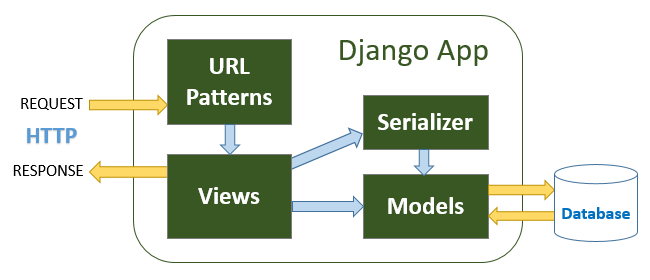
\includegraphics[width=110mm]{images/rest_flow.png}
    \caption{Modul de funcționare al Django REST Framework}
\end{figure}

Aplicația Voting App implementează toate conceptele de baze ale Django REST Framework. În primul rând au fost create modelele necesare pentru a susține un proces electoral:

\begin{itemize}
    \item User. Reprezintă clasa de bază a unui utilizator și conține datele acestuia - identificator, nume, prenume, email și grupul din care face parte. De asemenea, pe lângă aceste date, modelul User conține și structuri tip \enquote{boolean} pentru salvarea informațiilor cu vedere la rolurile pe care acesta le are - \enquote{admin}, \enquote{staff} sau \enquote{superuser}.
    \item Group. Acest model are la bază câmpuri pentru identificator, nume, descriere și culoare. Mai mulți utilizatori fac parte dintr-un grup, iar un singur utilizator nu poate face parte din două sau mai multe grupuri în același timp.
    \item Election. Este cea mai complexă clasă din Voting App, dat fiind necesitatea creării unui sistem cât mai customizabil și flexibil de votare. Acesta are câmpuri pentru \enquote{owner}, titlu, descriere, data începerii votului, data încheierii votului, data la care acesta a fost arhivat și variabile de tip \enquote{boolean} pentru a menține starea - \enquote{is\_active} și \enquote{is\_archived}. De asemenea mai are două câmpuri variabile, unul în care memorează numărul de întrebări din buletinul de vot și unul în care memorează grupurile de utilizatori care iau parte la procesul electoral.
    \item Question. Reprezintă o întrebare pusă într-un buletin de vot, aceasta putând apărea într-un număr aproape nelimitat pentru un singur proces electoral. Conține câmpuri pentru titlu, descriere și, în funcție de tipul întrebării (\enquote{single choice} sau \enquote{multiple choice}) schimbă valorile de opțiuni minime și maxime pe care un participant la vot le poate selecta.
    \item Option. Conține valoarea unei opțiuni din cadrul unei întrebări.
    \item Vote. Asemenea unei ștampile puse pe un buletin de vot, clasa Vote conține date despre opțiunea aleasă la o întrebare de către utilizator și procesul electoral la care acesta a luat parte.
    \item Submission. Pentru a putea vedea ce utilizatori au votat sau nu, clasa Submission funcționează drept un registru în care sunt adăugate date atunci când utilizatorul și-a exprimat votul. Această clasă nu memorează opțiunile alese de către utilizator, ci doar dacă acesta a votat sau nu la un anumit proces electoral.
\end{itemize}

De asemenea, pentru a arhiva un proces electoral încheiat, a fost realizat modelul \enquote{ClosedElection} cu scopul de a salva o copie a datelor finale pentru a le putea arhiva și pentru a putea fi mai ușor de accesat mai târziu. Acesta conține o referință la procesul inițial și un câmp JSON în care sunt salvate toate datele aferente.

În al doilea rând, Voting App se folosește de serializatoare pentru a transforma datele în format JSON astfel încât să fie transmise unui request. Aceste serializatoare au fost realizate pentru toate modelele declarate.

\begin{code}
\begin{minted}[bgcolor=bg,frame=lines,framesep=2mm,fontsize=\footnotesize,baselinestretch=1]{python}
class UserSerializer(serializers.ModelSerializer):
    group = GroupSerializer(many=False, read_only=True)
    class Meta:
        model = User
        fields = ['id', 'email', 'first_name', 'last_name', 'group', 'date_joined', \
            'last_login', 'is_staff', 'is_active']
\end{minted}
\captionof{figure}{Exemplu de serializator pentru modelul User}
\label{code:serializer-code}
\end{code}
\hfill

Avantajele folosirii serializatoarelor integrate în Django REST Framework este acela că permit un mod de utilizare foarte modular, dezvoltatorul putând să decidă ce câmpuri să includă sau să excludă.

\hfill

Nu în ultimul rând, pentru a putea lucra cu modelele și serializatoarele create, au fost implementate \enquote{View-uri}. Acestea au rolul de a procesa request-ul primit printr-o rută, adică, în Django, printr-un Url. Url-urile nu sunt nimic mai mult decât declarații ale rutelor prin care un client poate apela API-ul și, în funcție de request-ul făcut, execută View-ul atribuit. Url-urile pot primi un număr nedefinit de parametrii. Pentru Voting App, cele mai multe rute au primit ca parametru identificatorul obiectului pe care clientul dorește să îl acceseze

\begin{code}
\begin{minted}[bgcolor=bg,frame=lines,framesep=2mm,fontsize=\footnotesize,baselinestretch=1]{python}
    path('elections/<str:pk>/submit/', views.submitVotes),
    path('elections/<str:pk>/submissions/', views.getElectionSubmissions),
    path('elections/active/', views.getActiveElections),
    path('elections/inactive/', views.getInactiveElections),
    path('elections/<str:pk>/groups/', views.getGroupsFromElection),
    path('elections/<str:pk>/close/', views.closeElection),
\end{minted}
\captionof{figure}{Exemplu de Url-uri pentru modelul Election}
\label{code:url-code}
\end{code}
\hfill

În Voting App au fost folosite două tipuri de View-uri: de sine stătătoare și \enquote{ViewSet-uri}. View-urile de sine stătătoare sunt funcții ce nu aparțin unei clase și în care dezvoltatorul trebuie să specifice tipul request-ului (GET, POST, etc.) prin adnotarea \enquote{@api\_view}. De asemenea, pentru a adăuga un strat în plus de securitate, a fost folosită adnotarea \enquote{@permission\_classes} pentru a permite numai anumitor roluri de utilizator să acceseze View-ul.

\begin{code}
\begin{minted}[bgcolor=bg,frame=lines,framesep=2mm,fontsize=\footnotesize,baselinestretch=1]{python}
@api_view(['GET'])
@permission_classes([IsAdminUser])
def getActiveElections(request):
    elections = Election.objects.filter(is_active=True)
    serializer = MultipleElectionSerializer(elections, many=True)
    return(Response(serializer.data))
\end{minted}
\captionof{figure}{Exemplu de View care întoarce procesele electorale active}
\label{code:view-code}
\end{code}
\hfill

Pentru a gestiona mai ușor operațiile de tip CRUD, am folosit, în Voting App, ViewSet-uri \cite{what_is_viewset}. Acestea sunt clase atribuite unui model ce permit implementarea rapidă a operațiilor și prezintă metode pentru request-urile GET, POST, UPDATE, PATCH și DELETE. Au fost folosite ViewSet-uri pentru modelele User, Group, Election și ElectionSet.

\subsection{PyJWT}

PyJWT este o librărie de Python ce permite decodarea și codificarea de JSON Web Tokens (JWT). Aceste token-uri reprezintă un standard în industrie și definesc un mod ușor pentru a transmite, securizat, de cele mai multe ori, date între un client și un server \cite{what_is_pyjwt}. Ele permit autorizarea unui client atunci când acesta face un request din API și au următoarea structură \cite{what_is_jwt}:

\begin{itemize}
    \item Header. Conține două elemente - tipul token-ului (în acest caz JWT) și algoritmul de \enquote{signing} folosit (deseori SHA256, HMAC sau RSA).
    \item Payload. Este alcătuit din trei elemente: \enquote{Registered claims}, \enquote{Public claims} și \enquote{Private claims}. Aceste \enquote{claim-uri} conțin date precum: data de expirare a token-ului, identificatorul unui utilizator, datele personale ale acestuia, și nu numai. 
    \item Signature. Pentru a crea o semnătura se folosește header-ul codificat, payload-ul codificat, un \enquote{secret} și algoritmul specificat în header și se semnează.
\end{itemize}

În Voting App, a fost folosit PyJWT pentru a genera token-uri de autorizare atunci când un utilizator se autentifica cu succes. Aceste token-uri au fost folosite, în continuare, pentru a permite unui utilizator accesarea Url-urilor din aplicație, ele conținând identificatorul acestuia și data de expirare a token-ului.

\begin{figure}[!h]
    \centering
    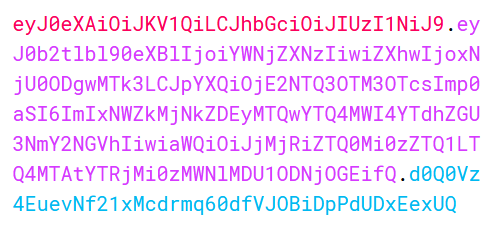
\includegraphics[width=110mm]{images/jwt_example.png}
    \caption{Exemplu de JWT folosit în Voting App}
\end{figure}

Într-un final, pentru a testa aplicația de backend, a fost folosită platforma Postman. Aceasta permite crearea de cereri HTTP și gruparea acestora într-un mod intuitiv. Au fost create cereri pentru toate Url-urile din aplicația de backend, fiind incluse și header-ele necesare.

\section{Baza de date}

\subsection{SQL}

Structured Query Language (SQL) este un limbaj de programare ce permite o interacțiune rapidă și eficientă din punct de vedere al timpului de execuție cu bazele de date. Acesta a fost dezvoltat de către inginerii de la IBM în anul 1974 și a rămas, încă de atunci, una dintre cele mai populare opțiuni atunci când vine vorba de dezvoltarea unei baze de date. Acest limbaj permite realizarea operațiilor de tip CRUD, fiind completat de o gamă variată de funcționalități precum: join-uri, indexări, operații matematice și nu numai.

\subsection{MySQL}

MySQL este un sistem open source de gestionare a bazelor de date relaționale, fiind creat de către Monty Widenius. Bazele de date relaționale stochează datele în tabele diferite, legate între ele prin chei de tip \enquote{foreign} \cite{what_is_mysql}. Pentru Voting App a fost folosit MySQL în scopul de a salva toate datele gestionate de către aplicația backend, astfel, fiind generate tabele, atât pentru modelele create cât și pentru cele \enquote{default}, necesare rulării Django și a librăriilor adăugate.

\begin{figure}[!h]
    \centering
    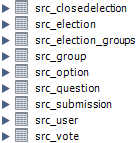
\includegraphics[width=45mm]{images/my_sql_example.png}
    \caption{Exemplu de tabele folosite pentru modelele din aplicația backend}
\end{figure}